\documentclass[a4paper,12pt,titlepage]{article}
\usepackage{tabularx}
\usepackage{tikz}
\usepackage{graphicx}

\graphicspath{ {img/} }

\renewcommand{\contentsname}{Inhoud}
\renewcommand{\figurename}{Figuur}

\begin{document}

\title{Schrumpke Sjieten \\ \large Het Offici\"ele Regelboek}

\date{7 Juni, 2015}
\author{Het Olympisch Comit\'e voor Schrumpke Sjieten\thanks{Met speciale dank aan Allaerts Dries, Driesen Joep en Somers Bran}}
\maketitle

\tableofcontents
\newpage

\section{Offici\"eel Jargon}

{\renewcommand{\arraystretch}{1.8}
\begin{tabularx}{\textwidth}{lX}

\textit{Een touw} & Een \textit{sjiet} waarbij de \textit{schrump} het touw raakt, er niet over valt en bijgevolg 3 punten oplevert voor de \textit{sjieter}. \\
\textit{Illegale Sjiet} & Een volledige \textit{sjiet} die niet volgens de offici\"ele sjiettechniek gebeurd. \\
\textit{Onvolledige Sjiet} & Een \textit{sjiet} waarbij de \textit{sjieter} voor het vervolledigen van de \textit{sjiet} door onvoorziene omstandigheden de \textit{schrump} op een minimale afstand achter de \textit{sjietlijn} laat vallen. \\
\textit{Overschrump} & Een \textit{sjiet} waarbij de schrump over het touw heen gaat. \\
\textit{Reschrump} & De tweede poging tot een volledige \textit{sjiet} na een \textit{onvolledige sjiet}. \\
\textit{Schrump} & Het spelvoorwerp waarmee gesjoten wordt (zie hoofdstuk \ref{sec:schrump}). \\
\textit{Schrumplijn} & De imaginaire lijn van de \textit{schrump} die het dichtste bij het touw ligt en nog meedingt naar het \textit{schrump point}.\\
\textit{Schrump Point} & Het punt dat toegekend wordt aan de speler wiens \textit{schrump} het dichtste bij het touw ligt zonder uit het spel verwijderd te zijn. \\
\textit{Schrump Set} & Een spelsituatie waarin een speler met zijn laatste \textit{sjiet} een nieuwe \textit{schrumplijn} gedefini\"eerd heeft. \\
\textit{Serve} & De eerste \textit{sjiet} in een ronde. \\
\textit{Sjiet} & Het werpen van een \textit{schrump} volgens de offici\"ele werptechniek (zie hoofdstuk \ref{sec:techniek}). \\
\textit{Sjieter} & De werper van een \textit{schrump}. \\
\textit{Sjietlijn} & De lijn waarachter elke \textit{sjieter} moet staan tijdens het \textit{sjieten} van zijn \textit{schrump}. \\
\textit{Underschrump} & Een \textit{sjiet} waarbij de \textit{schrump} onder het touw door gaat. \\

\end{tabularx}
}
\newpage

\section{De schrump} \label{sec:schrump}

De schrump is eender geconventioneerde kroonkurk met als origine de afsluiting van een glazen flesje bier. De kroonkurk dient een diameter van $3cm$ $(\pm 2mm)$ te hebben.

\begin{figure}[h]
\centering
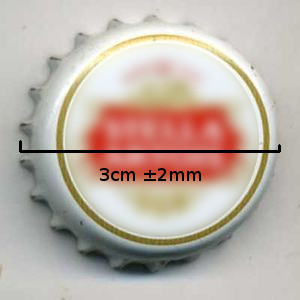
\includegraphics{schrump}
\caption{Een schrump die voldoet aan de offici\"ele voorwaarden (de sponsortext is in deze afbeelding onleesbaar gemaakt om neutraal te blijven over onze voorkeuren in bier).}
\label{fig:schrump}
\end{figure}

De schrump mag aan de bovenkant sponsortekst en -logo's bevatten.

\subsection*{Addendum juli 2007: Verzwaarde Schrumps}

Het is ten strengste verboden een schrump te verzwaren met inserts of andere middelen. Betrapt worden op verzwarende middelen zal leiden tot een directe diskwalificatie voor het evenement, een
verder onderzoek door de OCSS en mogelijk een permanente schorsing.

\newpage

\section{Het speelveld}

Er wordt steeds gespeeld op gras.

\begin{figure}[h]
\centering
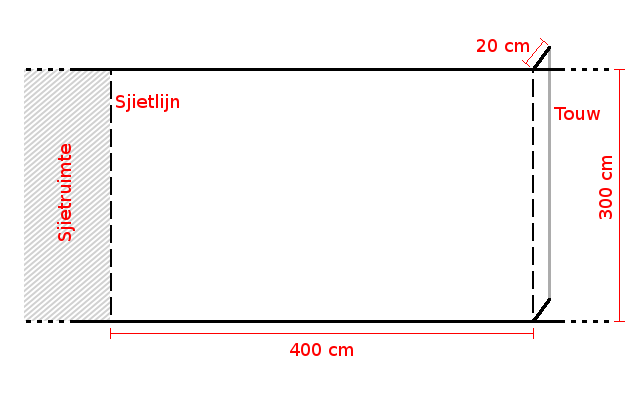
\includegraphics[width=\textwidth]{veld}
\caption{De opbouw en afmetingen van een officieel schrumpveld.}
\label{fig:veld}
\end{figure}

\newpage

\section{De werptechniek} \label{sec:techniek}

De schrump moet bovenhands (in een boog) gegooid worden. De schrump moet tijdens de worp gebalanceerd worden op de wijsvinger. De schrump klem zetten door de wijsvinger er om heen te buigen is 
verboden. De schrump zou als het ware van de vinger af moeten vallen indien de hand omgedraait wordt.

\newpage
\section{Het scoresysteem}

De spelers kunnen op 3 manieren punten verdienen:

\begin{enumerate}
\item Een speler wiens schrump het touw raakt (en er niet over gaat) scoort een 'touw'. \\Dit is 3 punten waard.
\item Een speler wiens schrump onder het touw gaat en volledig voorbij het touw belandt scoort een 'underschrump'. \\Dit is 2 punten waard.
\item Elke schrump die binnen het speelveld ligt en niet onder \'e\'en van voorgaande categori\"en valt, dingt mee naar het schrumppunt. Dit punt wordt op het 
      einde van de ronde toegekent aan de spelers wiens schrump het dichtste bij het touw ligt.
\end{enumerate}

Een spelers wiens schrump over het touw heen gaat, kan die ronde geen punten verdienen (ookal raakt hij het touw, hij dingt dus ook niet mee naar het schrumppunt).

\newpage

\section{De touwmeester}

\newpage



\section{Het Spelverloop}

\subsection{Bepaling van de sjietorde}

\begin{itemize}
\item Voor de eerste ronde van een spel sjieten alle spelers tegelijkertijd een schrump richting het touw. De speler wiens schrump het verste van het touw ligt, sjiet in de komende ronde eerst. De volgende
      schrump sjiet als tweede, etc.. In deze spelfase tellen ook schrumps die over het touw heen gaan mee.
 \item Voor elke volgende ronde sjieten spelers die in de vorige ronde een hoger aantal punten hebben behaald eerst. 
 \item Indien er een gelijk aantal punten behaald werd, sjiet de persoon die in de vorige ronde later was, nu eerder.
\end{itemize}

\subsection{Het sjieten}

De speler sjieten \'e\'en voor \'e\'en, in volgorde van de sjietorde, hun schrump richting het touw volgens de offici\"ele sjiettechniek. Tijdens deze ronde mogen de speler het veld niet voorbij de sjietlijn komen, noch deze
aanraken met de schoen. Het is voor de spelers die reeds gesjoten hebben wel toegelaten naast het speeldveld te gaan staan teneinde het verdere verloop van de ronde beter te kunnen waarnemen. 

Een speler mag de touwmeester steeds vragen een eerder gesjoten schrump aan te duiden in het geval deze niet duidelijk zichtbaar is.

Een schrump die over het touw heen gaat wordt voor de rest van de ronde niet meer beschouwt en de sjieter kan bijgevolg geen punten verdienen.

\subsection{Toekennen van de score}

Wanneer alle spelers gesjoten hebben, is het aan de touwmeester de score te bepalen (indien nodig het veld te betreden om metingen uit te voeren) en toe te kennen. Pas wanneer de touwmeester dit aangeeft, mogen de spelers
het veld betreden om hun schrump op te rapen.

Het is de spelers steeds toegestaan een hermeting aan te vragen indien er redelijk twijfel kan bestaan over het resultaat. Hierna staat de beslissing van de touwmeester echter buiten discussie.

\subsection{Einde van het spel}

Een spel bestaat uit meerdere ronden. Het spel eindigt wanneer een speler de winscore behaalt heeft en bovendien minstens 2 punten meer heeft dan de speler met de volgende hoogste score. De winscore wordt op voorhand
bepaald en aangekondigt door de organiserende instantie van het evenement. Het OCSS raadt echter volgende winscores aan naargelang de aard van het evenement:

\vspace{10mm}

\begin{table}[h]
\centering
\begin{tabular}{l|l}
Vriendschappelijk & 6 \\
Kampioenschap & 11 \\
Olympisch & 15 \\
\end{tabular}
\end{table}

\vspace{10mm}

Het is uiteraard ook toegestaan doorheen een evenement een variabele winscore te hanteren, zolang dit duidelijk aangekondigt is.


\end{document}